\ifx\boi\undefined\ifx\problemname\undefined
\providecommand\sampleinputname{}
\providecommand\sampleoutputname{}
\documentclass[english]{templates/boi}
\problemlanguage{.en}
\fi
\newcommand{\boi}{Baltic Olympiad in Informatics}
\newcommand{\practicesession}{Practice Session}
\newcommand{\contestdates}{April 27 - May 1, 2018}
\newcommand{\dayone}{Day 1}
\newcommand{\daytwo}{Day 2}
\newcommand{\licensingtext}{This problem is licensed under CC BY-SA 4.0.}
\newcommand{\problem}{Problem}
\newcommand{\inputsection}{Input}
\newcommand{\outputsection}{Output}
\newcommand{\interactivity}{Interactivity}
\newcommand{\grading}{Grading}
\newcommand{\scoring}{Scoring}
\newcommand{\constraints}{Constraints}
\renewcommand{\sampleinputname}{Sample Input}
\renewcommand{\sampleoutputname}{Sample Output}
\newcommand{\sampleexplanation}[1]{Explanation of Sample #1}
\newcommand{\sampleexplanations}{Explanation of Samples}
\newcommand{\timelimit}{Time Limit}
\newcommand{\memorylimit}{Memory Limit}
\newcommand{\seconds}{s}
\newcommand{\megabytes}{MB}
\newcommand{\group}{Group}
\newcommand{\points}{Points}
\newcommand{\limitsname}{Limits}
\newcommand{\additionalconstraints}{Additional Constraints}
\newcommand{\testgroups}{
Your solution will be tested on a set of test groups, each worth a number of points.
Each test group contains a set of test cases.
To get the points for a test group you need to solve all test cases in the test group.
Your final score will be the maximum score of a single submission.
}
\fi
\def\version{jury-1}
\problemname{Växelström}
Fredrik är hemma och leker med sin hemmabyggda modelljärnväg, som han är mycket stolt över.
Järnvägen består av $N$ segment som sitter ihop i en cirkel, numrerade $1, 2, \dots, N$ i medurs ordning.
Tåget får elektricitet från vajrar som leder längs cirkeln. Varje segment har minst en vajer som leder förbi det. 

Fredrik tycker att sitt cirkulära tåg börjar bli tråkigt, och istället för bestämmer sig för att lägga till en \emph{järnvägsväxel} till varje segment, vilket han kan använda för att skapa avspårningsolyckor och andra spännande scenarier.
Växlarna behöver dock elektricitet, och inte vilken elektricitet som hellst. 
De behöver växelström, strömmen som driver växlar.

Fredrik inser att sättet man får växelström på är att ha ström i båda riktningarna.
Varje varjer kan endast leda ström i en riktning, antingen medurs eller moturs, 
men Fredrik får bestämma riktningen. Han vill alltså bestämma strömriktning på vajrarna
så att varje segment är täckt av både en vajer med medurs strömriktning och en med moturs
strömrikting.

Kan du hjälpa Fredrik bestämma riktningarna?

\vspace{2mm}
%\hspace*{2mm}
\begin{center}
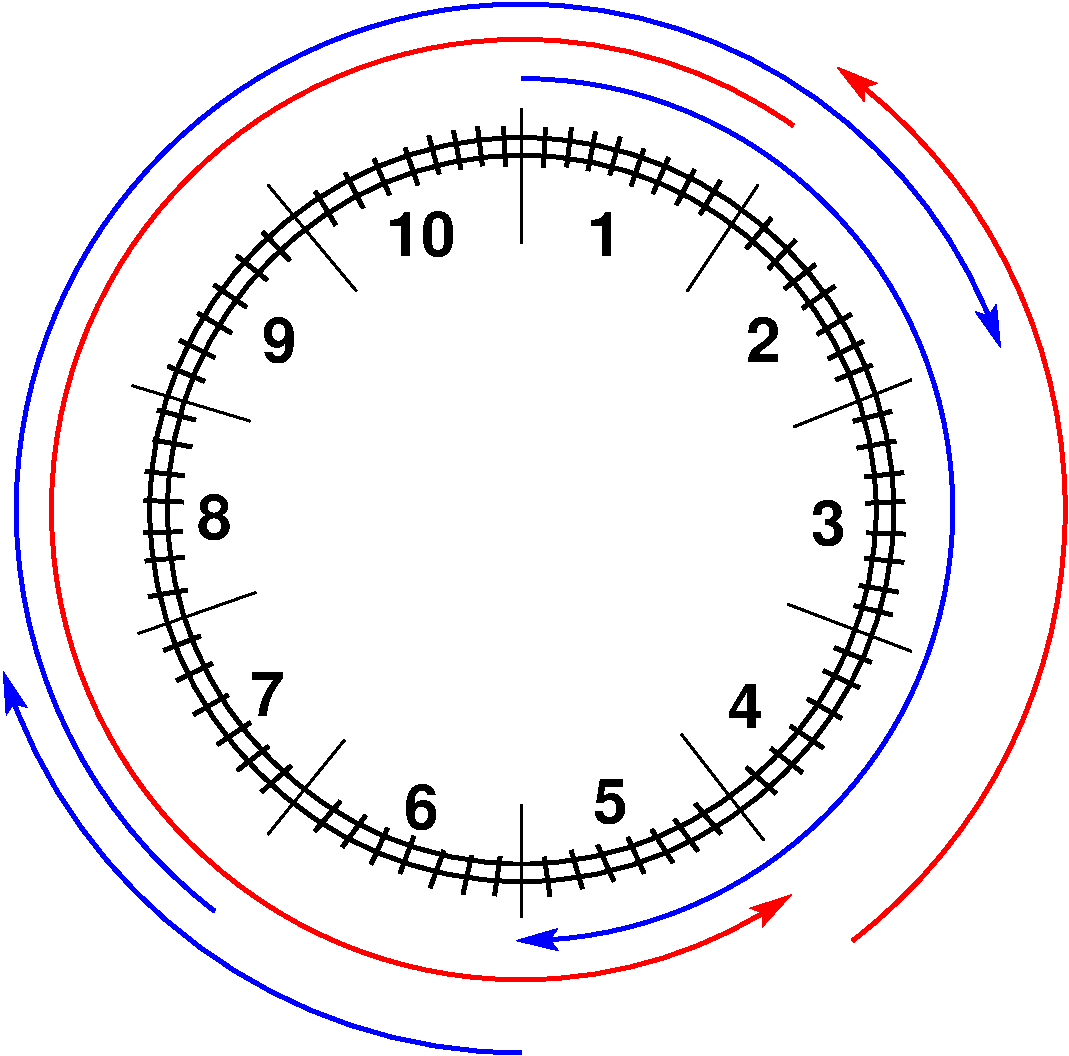
\includegraphics[width=0.5\textwidth]{alternatingfig.pdf}
\end{center}
\vspace{1mm}
{\em En lösning till det första testallet. De krökta pilarna utanför järnvägen representerar 
vajrar som leder ström. Rikningen på pilarna representerar Fredriks val av strömriktning (vilket förtydligas av blå och röda färger på pilarna). Notera att alla strömriktningar för kunde ha bytts för att få den andra giltiga lösningen: \texttt{11010}.}

\section*{\inputsection}
Den första raden innehåller två heltal $N$ och $M$, antalet järnvägssegment och antalet vajrar.

Nästa $M$ rader innehåller två heltal $1 \le a, b \le N$, vilket indikerar att det går en vajer förbi alla segment $a, a+1, \dots, b$. Om $b$ är mindre än $a$ går vajern förbi segmenten $a, a+1, \dots, N, 1, \dots, b$. Notera att om $a=b$ går vajern bara förbi ett segment.

\section*{\outputsection}
Skriv ut en enda rad med $M$ tecken, vilka är antingen \texttt{0} or \texttt{1}. Det $i$:te tecknet ska vara \texttt{0}
om den $i$:te vajern i indatan har medurs strömriktning, medan tecknet ska vara \texttt{1} om vajern har moturs strömriktning.
Om det finns många lösningar kan du skriva ut vilken som av dem.

Om det är omöjligt att välja strömriktning på vajrarna så att varje segment täcks av en med medursriktad ström och en med motursriktad ström, skriv ut ``\texttt{impossible}''.

\section*{\constraints}
\testgroups

\noindent
\begin{tabular}{| l | l | l | l |}
\hline
\textbf{\group} & \textbf{\points} & \textbf{\limitsname} & \textbf{\additionalconstraints} \\ \hline
  1     & 13     & $2 \le N, M \le 15$ & \\ \hline
  2     & 20     & $2 \le N, M \le 100$ & \\ \hline
  3     & 22     & $2 \le N, M \le 1000$ & \\ \hline
  4     & 19     & $2 \le N, M \le 100\,000$ & Ingen vajer har $b < a$. \\ \hline
  5     & 26     & $2 \le N, M \le 100\,000$ & \\ \hline
\end{tabular}

